%%=============================================================================
%% Inleiding
%%=============================================================================

\chapter{Inleiding}
\label{ch:inleiding}

Security is de laatste jaren een echte trend geworden. Elk bedrijf is hiermee bezig, en ook in het nieuws komen er steeds meer berichten over beveiliging. Maar hoe zou een bedrijf hier zich best tegen kunnen verdedigen? Is een gewone firewall en antivirus niet genoeg meer?

De volgende stap is voor vele bedrijven een 'Vulnerability management' systeem. Dit is een continu proces dat bestaat uit 4 delen:  'discovery', 'reporting', 'prioritization' en 'response'. Tijdens het 'discovery' deel moet ELK systeem getest worden en in een databank geplaatst worden. Deze databank wordt gebruikt in de volgende stap 'reporting'. Hier moet er een rapport gemaakt worden zodat alle risico's in kaart gebracht kunnen worden. Eens dat de rapporten klaar zijn, moeten er 'priorities' opgesteld worden. Dit gebeurt door elk risico te bekijken en studeren wat de invloed is op het netwerk als deze misbruikt word. Uiteindelijk moeten deze risico's opgelost worden in het 'response' deel. \textcite{Tripwire}

Voor we beginnen uitleggen wat men hiervoor kan doen als verdediging, zuller er een paar termen uitgelegd worden dat essentieel zijn voor het verdere verloop van dit onderzoek. Een vulnerability is een zwakheid in een stuk code of een design fout (de meeste vulnerabilities komen van verouderde software en verkeerd geconfigureerde software) waardoor het mogelijk is om een actie uit te voeren wat niet de intentie van de software en/of het design was \textcite{Techtarget-vuln}. Vulnerabilities die het mogelijk maken om informatie te krijgen van het systeem krijgen een CVE nummer. Dit is een uniek nummer voor een publieke vulnerability dat begint met het jaar waarin deze ontdekt werd. Deze nummers en namen zijn nodig omdat voor dit systeem bestond, elk bedrijf een andere naam had voor een vulnerability. Dit was onduidelijk en zorgde voor veel verwarring \textcite{cve-mitre}. De acties dat gebruik maken van een vulnerability om bepaalde commandos uit te voeren op een machine (Arbitrary code execution) of een server niet meer toegankelijk maken voor legitieme gebruikers (Denial of Service), noemen we exploits \textcite{Techtarget-exploit}.

Tools dat voor vulnerability management gebruikt kunnen worden noemen we scanners. In dit onderzoek zal ik alleen de 'Vulnerability scanners' bespreken. Dit is een beveiligingstechniek  dat fouten in een systeem kan opsporen \textcite{Techopedia} over een netwerk. Deze tools worden zowel gebruikt door 'black hats' als 'white hats'. Het verschil tussen deze 2 is dat de 'white hat' ethisch correct is. Deze zal op voorhand toegang vragen om een systeem te mogen testen, en als deze test lukt het bedrijf melden wat er mis is. De 'black hat' vraagt geen toestemming en gebruikt de testen om binnen te dringen op een systeem en de data hiervan te verkopen, of het systeem te laten crashen \textcite{Howtogeek}. Voor een volledig vulnerabiliy management bij te houden, moet men ook nog andere scanners implementeren zoals een 'web application scanner' (bv. Arachni). Deze scant een website op mogelijke problemen als SQL injecties en cross-site scripting. 

Een SQL injectie, is een vulnerability dat voorkomt als men data moet invullen op een website dat een actie uitvoert op de databank. Deze kunnen gaan van een wachtwoord van een gebruiker omzeilen, tot toevoegen of verwijderen van data \textcite{acunetix}.

Cross-site scripting (vaak afgekort als XSS), is een techniek waarbij een hacker legitieme gebruikers kan aanvallen via een legitieme website. Deze techniek wordt vooral misbruikt bij javascript, omdat deze op bijna elke site aanwezig is. Dit gebeurt als er input van een gebruiker gebruikt wordt door bijvoorbeeld HTML of JS. Hier kan de aanvaller de gebruiker bijvoorbeeld doorverwijzen naar een valse website, en daar persoonlijke data van de gebruiker proberen te krijgen \textcite{acunetix-xss}.

Het resultaat van een vulnerability scan is meestal een lijst met 'cvss' scores van de gescande targets. Een cvss score is een framework om te bepalen hoe erg een bepaalde vulnerability is. Dit word bepaald door een complexe formule waarbij er rekening gehouden wordt met de impact op de target server, welke privileges je op de server reeds moet hebben, hoe complex de vulnerability is en van waar deze vulnerability misbruikt kan worden (lokaal netwerk, internet, fysische toegang, ...). Deze scores liggen tussen 0 en 10 en hebben aan de hand hiervan een bepaald label. Volgens versie 3 van cvss zijn de labels: low (0-3.9), medium (4-6.9), high (7-8.9) en critical (9-10) \textcite{Nist}. Naast een cvss score, heeft het rapport ook een oplossing voor de vulnerability (indien deze bestaat). Deze kan bestaan uit het updaten van een bepaalde service, tot een configuratie file aanpassen.

Momenteel zijn er een aantal vulnerability scanners, maar voor dit onderzoek zal er alleen rekening gehouden worden met 'openvas' en 'nessus'. De reden hiervoor is dat nessus momenteel 1 van de populairste en bekendste tools hiervoor is dankzij zijn kwaliteit/kost verhouding \textcite{Sectools}, maar deze heeft voor bedrijven wel een betalende licentie nodig \textcite{Tenable}. Openvas daarintegen is open-source en is gebaseerd op de laatste code die van nessus is vrijgegeven. Hierdoor kunnen we ook vergelijken of het mogelijk is om een open-source security producten te gebruiken in plaats van betalende software, en of deze dezelfde kwaliteit kan leveren. 

Hoewel dit niet de primaire bedoeling is van dit onderzoek, is dit wel een mooie toevoeging. Een andere scanner die in aanmerking kwam voor dit onderzoek was CORE impact, deze wordt gezien als een van de beste en meest volledige scanners. De reden waarom deze niet onderzocht geweest is, is omdat deze een zeer hoge licentiekost heeft, en geen gratis versie heeft dat we konden gebruiken voor dit onderzoek.

\section{Stand van zaken}
\label{sec:stand-van-zaken}

In het volgende deel zal ik meer uitleg geven over hoe vulnerability scanners werken, ook refereer ik naar gelijkaardige onderzoeken en wat de verschilpunten zijn met mijn onderzoek. Hierna geef ik meer uitleg over nessus en openvas zelf, en wat de theoretische verschillen hiertussen zijn (zoals licenties,hardware,...).  De praktische verschillen zullen we in het volgende hoofdstuk bespreken.

Elk onderzoek dat verband heeft met security is nooit lang up-to-date. Dit komt omdat deze constant veranderd en er steeds nieuwe technieken worden ontdekt waar men zich moet tegen beschermen. Een interessant voorbeeld van deze innovatieve technieken is over \textcite{Linkedin}. Hierin slaagde een persoon om met css (Cascading Style Sheet), een webpagina van linkedin over te nemen. Dit werd mogelijk gemaakt door een bestaand css regel dat het hele scherm in gebruik nam. De aanvaller gebruikte via injecties deze regel om het hele scherm aanklikbaar te maken, en naar een wilkeurige site te gaan.

Dit onderzoek is hier dus geen uitzondering. Na een paar maanden zal sommige informatie irrelevant zijn. Dit wil zeggen dat ook vorige onderzoeken al oude informatie kunnen gebruiken, waardoor men zich hierop niet kan baseren.

\subsection{Gelijkaardige onderzoeken}
%todo: dit stuk mss wat herschrijven? + verklaren van woorden

Volgens de meeste onderzoeken die gevoerd zijn, is core impact de 'beste' scanner. Hiermee wordt bedoeld dat deze zeer snelle updates heeft met NVTs en een aantal tools ingebouwd heeft voor 'false positives' te testen, maar de licentiekosten bedragen rond de 30.000\$ / jaar. De meest populaire is zoals eerder vermeld nessus. \textcite{Concise} \&\& \textcite{Sectools} 

Voor een vergelijking tussen openvas en nessus, is het aantal papers beperkt. Men geeft steeds dezelfde links naar het onderzoek \textcite{Hackertarget}. Dit onderzoek is gebeurt rond Juni 2012, voor security standards is dit dus heel outdated. Hoewel de vergelijking goed beschrijft hoe de scans gebeurt zijn en in welke environment dit gebeurt is, zijn er een aantal zaken die ontbreken. Zoals bijvoorbeeld een windows target. In het onderzoek heeft men alleen metasploitable gebruikt. Ook waren de 'extra' tools voor openvas niet geinstalleerd en werd voor de nessus scan niet een volledige diepe scan uitgevoerd. In de comments werd het nessus probleem aangesproken door Paul Asadoorian. Deze werkt voor tenable en heeft een uitleg gegeven hoe je een volledige scan doet met nessus \textcite{Securityweekly}. Merk op dat deze referentie partijdig is, sinds deze gegeven werd door een medewerker van nessus.

Een ander onderzoek \textcite{Rageweb} gebruikt wel windows en linux targets, maar geeft geen informatie over hoe alle scans uitgevoerd zijn. Dit is een groot probleem als men niet voor elke scanner een gelijkaardig profiel gekozen heeft. Wel is dit onderozek interessant omdat er een methode gebruikt werd om 'false positives' eruit te filteren. Deze is helaas niet meer beschikbaar in de huidige versie van metasploitable, en is dus ook niet meer toepasbaar op dit onderzoek.

Andere gevoerde onderzoeken werden uitgevoerd als nessus nog open source was en zijn dus ook niet toepasbaar op dit onderzoek, of waren van een te lage kwaliteit om deze te analyseren. 

\subsection{Hoe werkt een vulnerability scanner}

%TODO: verwijzen naar bijlage voor een stuk code van een NVT (openvas source code)

Een vulnerability scanner bestaat traditioneel uit 3 delen. Een user interface, een manager en een scanner. Eerst zal er een kleine uitleg gegeven worden over hoe alle delen met elkaar werken, en daarna een gedetailleerde beschrijving hoe een target gescanned word.

%todo bronvermelding!
\begin{figure}[h]
\caption{Vulnerability scanner structuur}
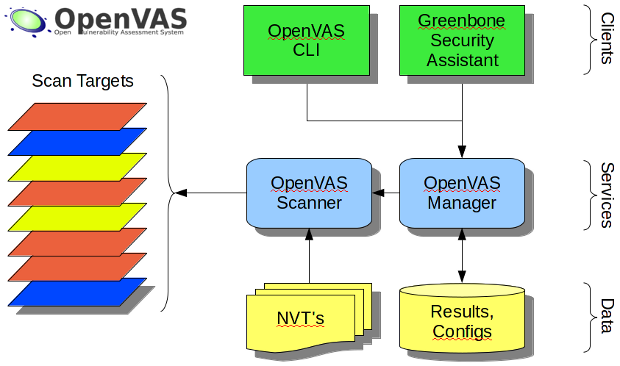
\includegraphics[width=10.0cm]{img/Openvas-structuur.png} \textcite{Openvas-about}
\end{figure}
 
De user interface (hierboven vermeld als 'Greenbone Security Assistant') is in veel gevallen een webinterface dat acties doorstuurt naar de manager, zoals een scan starten, of rapporten maken. Het is ook mogelijk om acties door te sturen naar de manager via een command line interface (hierboven vermeld als 'OpenVAS CLI'), dit is handig voor als men scans wil automatiseren.

De manager (hierboven vermeld als 'OpenVAS Manager') staat in voor de communicatie tussen de user interface en de scanner engine. Deze onderhoud ook een aantal databanken waarin alle configuraties, resultaten, SCAP data, CERT data en NVT's zitten. SCAP, CERT en NVTs zijn hierbij de belangerijkste, deze staan in voor het testen van een target of deze vulnerable is. SCAP data is een feed waarbij de community helpt deze te ontwikkelen \textcite{whatis-scap}. Het verschil met CERT data is dat deze eerder voor interne scans bedoeld is, door een serie van testen uit te voeren met een aangemelde gebruiker \textcite{whatis-cert}.Uiteindelijk zijn er nog NVTs, deze zijn geen vaste feeds waar iedereen dezelfde data krijgt. Deze hangt af per vulnerability scanner. Later in dit onderzoek zullen we deze verschillen duidelijk zien met openvas en nessus. Het is de job van de manager om deze databanken up-to-date te houden zodat deze steeds een volledige vulnerability management oplossing kan bieden.

De scanner (hierboven vermeld als 'OpenVAS Scanner') staat in voor de effectieve scan van een target. Deze heeft een cache waar alle NVT's aanwezig zijn die de scanner nodig heeft om een target te kunnen scannen. Deze geeft zijn resultaten terug aan de manager. 

Indien men een scan start voor een range van machines, zal de scanner engine eerst een 'alive check' uitvoeren op alle hosts in de range. Dit kan bestaan uit een simpele ICMP ping naar de host, tot een range van poorten scannen en kijken of de host reageert op 1 van de requests. 

Indien de host reageert, zal er een port scan gestart worden, de tool die men hiervoor gebruikt is in veel gevallen 'nmap'. De range van poorten wordt op voorhand gedefinieerd door de gebruiker en indien er een firewall aanwezig is, zal hier ook rekening mee gehouden worden. 

De scanner zal hierna een aantal dingen analyseren, zoals het besturingssysteem dat op de host draait, en welke services overeen komen met de open poorten. Als al deze feiten uiteindelijk bekend zijn, zal de scanner op basis van deze analyse NVTs naar de hosts sturen en kijken of deze vatbaar is voor bepaalde exploits \textcite{Qualys}.

Uiteindelijk zal de scanner alle gevonden informatie doorsturen naar de manager, en op basis hiervan een rapport maken die leesbaar is voor de gebruiker.

\subsection{Requirements}

%TODO: wat beter herschrijven
%TODO: functionaliteiten opsommen!

In de volgende delen, zullen we nessus en openvas vergelijken op een aantal vlakken dat belangerijk zijn in een scanner. Een aantal belangerijke zaken (snelheid van de scanner, accuraatheid, etc...) zullen pas besproken worden in hoofdstuk~\ref{ch:methodologie}, omdat deze tot het onderzoek behoren. Eerst zal er kort een aantal zaken besproken worden zoals de geschiedenis van de scanner, de licenties, de support dat de scanner krijgt en de hardware vereisten. Hierna bespreken we de belangerijkste zaken.

Een volwaardige vulnerabiltiy scanner moet aan een paar voorwarden voldoen, het belangerijkste onderdeel zijn de NVTs. Als deze niet tijdig worden geüpdate, is de scanner niet meer betrouwbaar voor de nieuwste vulnerabilities, en geeft dit een vals veilig gevoel. Hiervoor zullen we 2 grote vulnerabilities (1 voor linux, en 1 voor windows) opzoeken en kijken wanneer beide scanners deze NVT toegevoegd hebben. Voor linux heb ik gekozen voor de 'shellshock' vulnerability (CVE-2014-6271), voor windows is dit 'Server Service Vulnerability' (CVE-2008-4250)

Uiteindelijk bespreken we ook de functionaliteiten van beide scanners. Eerst zullen we bepaalde funtionaliteiten bespreken die een betere performantie geven, of een accurater beeld geven van het systeem. Daarna bespreken we bepaalde functies die niet direct bijdragen tot het eindrapport, maar de scanner gemakkelijker laten implementeren met de bestaande infrastructuur of het grootste deel van het onderhoud automatiseren. 

%TODO: meer testen toevoegen dat impact hebben op eindrapport
Voor het eerste deel gaan we na of beide scanners een 'credential scan' ondersteunen, deze test gebeurt door het inloggen op een bepaalde dienst (meestal ssh) en heeft dus ook de mogelijkheid om configuratie files te controleren op fouten \textcite{Digitalbond}. Een basisvereiste is ook vaak dat scanner meerdere scans tegelijkertijd kunnen uitvoeren, Hoewel dit bij moderne scanners zo goed als steeds het geval is gaan we voor volledigheid dit ook nakijken. Uiteindelijk kijken we ook of de scanner 'agent based' scanning toestaat, dit is een klein programma dat op een host geïnstalleerd word, en commandos van van een centrale machine kan ontvangen. Deze zal een scan uitvoeren op de lokale machine, en zijn resultaten doorsturen naar de centrale machine waar deze beschikbaar is via alle interfaces.

%TOOD: meer testen toevoege ndat GEEn impact hebben op eindrapport 
%TODO: RESP/API uitleggen
Uiteindelijk kijken we of  de server zichzelf onderhoud (zoals NVTs updaten), en wat er nog manueel moet gebeuren. Ook kijken we of er een REST interface, of een API aanwezig is. Hierdoor is het mogelijk om acties uit te voeren op de scanner server, zonder enige extra software te moeten installeren op het systeem.
%---------------------------------------------------

\subsection{Nessus}

%TODO: informatie over nessus (prijs,tennable, geschiedenis, edities, support, etc...
%TODO: history citen naar boek V werkt niet voor een reden
%@BOOK{Nessus,
%  TITLE = {Nessus Network Auditing},
%  AUTHOR = {Carey Mark, Russ Roger, Paul Criscuolo, Mike Petruzzi},
%  YEAR = {2008}, 
%  PUBLISHER = {O'reilly},
%}

\subsubsection{Geschiedenis}
Nessus is in 1998 opgericht door Renaud Deraison, met de bedoeling om een gratis vulnerability scanner te maken dat over het internet machines kon scannen. Rond deze software werd het bedrijf tenable opgericht en werd al snel 1 van de populairste oplossingen voor vulnerability managment. Vanaf nessus versie 3 (2005) werd de source code niet meer publiek gemaakt omdat er misbruik van gemaakt werd door de concurrentie. De nessus scanner werd doorverkocht door bedrijven met hun eigen logo en vermelden dat het hun scanner was, ook was er weinig tussenkomst van de community (vooral op gebied van de scanner engine) \textcite{Cnet}.

\subsubsection{Licenties}
Tenable heeft een aantal nessus producten, maar voor dit onderzoek kijken we naar 'Nessus Professional'. De reden hiervoor is dat dit product zo goed als volledig overeenkomt met een openvas installatie (met een paar limitaties). De licentiekosten hiervoor zijn 2190 \$ / jaar (ongeveer 2010 euro) en is proprietary software.
 
\subsubsection{Support}
Als men een licentie van 'Nessus Professional' heeft, is het mogelijk om support te krijgen via live chat, email en een support portal. Deze zaken zijn 24/7 te benaderen \textcite{Nessus-support}.
 
\subsubsection{Nvt development}
Nessus heeft op moment van schrijven 87.071 plugins \textcite{Nessus-nvt}. Deze NVTS worden geschreven in .nasl (Nessus attack script language).

Voor de shellshock vulnerability is er een NVT verschenen op 24-09-2014 \textcite{Vulners-shellshock-nessus}. Dit is dezelfde dag als shellshock publiek gemaakt werd. De windows vulnerability NVT werd geüpload op 23-10-2008, dit is ook op de dag dat windows de vulnerability publiek maakte.
 

\subsubsection{Functionaliteiten}
\textbf{\textit{Credential scan: }} Deze functionaliteit is beschikbaar, met ondersteuning voor een aantal services. De belangerijste services worden hier opgelijst: database, mongoDB, ssh, windows en SNMPv1/v2c \textcite{Nessus-functions}.

\textbf{\textit{Meerdere scans: }} Dit is mogelijk op elke versie.

\textbf{\textit{Agent based: }} Dit is niet mogelijk met de 'professional' licentie, maar wel met de 'manager' licentie \textcite{Nessus-functions}.
%todo: kijken of nessus cron gebruikt
\textbf{\textit{Onderhoud: }} Op de webinterface is het mogelijk om bepaalde of alle  elementen te updaten. Ook is het mogelijk om een interval in te stellen wanneer deze moet geüpdate worden (dagelijks, wekelijks of maandelijks).

\subsubsection{Hardware}
De minimum systeemvereisten voor een scanner zijn:

\begin{itemize}
\item Dual core 2GHz CPU
\item 2-4 GB RAM
\item 30GB HDD
\end{itemize}

\textcite{Nessus-requirements}

%-------------------------------------------------------------------

\subsection{Openvas}

\subsubsection{Geschiedenis}
Openvas is een fork van de laatste source code die nessus publiek heeft gemaakt in 2005, en begon onder de naam \textcite{Securiteam} en werd opgestart door Tim Brown. Dit project is nog steeds volledig opensource \textcite{Openvas-source} en gratis voor zowel personen, als bedrijven met uitzondering op een (niet verplichte) betalende licentie van greenbone voor NVT's \textcite{Openvas-nvt}. De grootste bijdrager voor openvas is greenbone, deze zorgt voor een groot deel van de NVTs, de webinterface en bugfixes \textcite{Openvas-contributors}.

\subsubsection{Licenties}

Openvas valt onder de GPL license, is open-source en is gratis te gebruiken voor zowel personen, als bedrijven.

\subsubsection{Support}

Een nadeel van open-source projecten is vaak dat je afhankelijk bent van de community voor support. Dit is bij openvas niet anders, buiten een mailing list en een IRC is de support zo goed als niet bestaande. Een 'Internet relay chat (IRC)' is een online chatroom waar een reeks gebruikers zich aanmelden om over een bepaald onderwerp te Discussiëren \textcite{IRC}. In dit geval is het onderwerp openvas, en heeft de IRC gemiddeld 2000-3000 lijnen per uur \textcite{Openvas-IRC}. Een mailing list is een lijst van mensen die zich met een email geabonneerd heeft. Hier verstuurt een andere gebruiker of bedrijf een email naar over een bepaald onderwerp zodat deze mensen up-to-date blijven met alle nieuwigheden. Een voorbeeld hiervan is de openvas mailing list, deze verstuurt een mail telkens dat er een nieuwe versie beschikbaar is. Deze mail bevat alle informatie met wat er veranderd is ten opzichte van de vorige versie \textcite{techtarget-mailinglist}.

De openvas website bevat veel verouderde links zoals een wiki en een aantal screenshots. Op het moment van schrijven is de laatste entry in de wiki voor openvas 7 \textcite{Openvas-wiki}, ook op de screenshots pagina is de laatste entry voor openvas 7 \textcite{Openvas-screenshots}.

\subsubsection{Nvt development}

Openvas heeft op het moment van schrijven 53.082 plugins \textcite{Openvas-nvt} waarvan er 214 geüpload zijn in de laatste maand. Wat hier ook opvallend is, is dat alle plugins in openvas geschreven worden in nasl (dit staat voor 'nessus attack script language'). Openvas gebruikt dus nog steeds dezelfde code voor NVTs te schrijven als nessus. 

Voor de shellshock vulnerability heeft openvas de NVT geupload op 25-09-2014 \textcite{Vulners-shellshock-openvas}. Dit is 1 dag later als de announcement van shellshock en is gemaakt door greenbone. Dit lijkt onschuldig, maar shellshock heeft 24 uur na de ontdekking al voor het ontstaan van botnets gezorgd \textcite{wired-shellshock}. 

De windows vulnerability werd beschikbaar gesteld op 24-10-2008, Dit is 1 dag na de bekendmaking door windows. Hoewel de gevolgen niet zo erg waren als shellshock, gebruikte de worm \textcite{Microsoft} deze vulnerability om zich te verspreiden. Een worm is een stuk software dat zichzelf automatisch kan verspreiden, waarbij het meestal leidt tot het installeren van backdoors of data kan stelen van een gebruiker \textcite{pctools-worm}. Een backdoor is een techniek waardoor het mogelijk wordt om een prompt te krijgen op een systeem zonder dat de gebruiker hiervan weet \textcite{techopedia-backdoor}.

\subsubsection{Functionaliteiten}

\textbf{\textit{Credential scan: }} Deze functionaliteit is beschikbaar, maar dit is niet op scan niveau. Dit betekent dat men 2 verschillende targets (systeem dat gescanned zal worden) moet aanmaken als men een credential en een non-credential wil starten (ookal is dit hetzelfde IP). De ondersteunde services zijn hier: SSH, SMB, ESXi en SNMP.

\textbf{\textit{Meerdere scans: }} Dit is mogelijk.

\textbf{\textit{Agent based: }} Dit is mogelijk.

\textbf{\textit{Onderhoud: }} Het is niet mogelijk om in de webinterface updates te starten. De updates (voor alles) worden wel automatisch elke dag geüpdate om 1 uur snachts door middel van cronjobs. Crond is een daemon dat draait op de achtergrond en dat toestaat op een bepaald interval een actie uit te voeren indien de gebruiker hier permissies voor heeft \textcite{adminschoice}. Deze kan gebruikt worden voor bijvoorbeeld gegevens op te halen, of in het geval van puppet op een bepaald interval een puppet run te starten.

\subsubsection{Hardware}
De minimum systeemvereisten voor openvas staan niet op de site, er is wel een virtuele machine aanwezig voor openvas te testen. De requirements hieronder zijn van deze virtuele machine, in realiteit zullen deze requirements hoger liggen. De reden hiervoor is dat dit een minimale versie is dat bepaalde features niet heeft, ook zijn er nog meer beperkingen zoals dat het besturingssysteem kan niet updaten. Dit is dus niet gepast voor een productie omgeving.

\begin{itemize}
\item Dual core CPU
\item 2 RAM
\item 9GB HDD
\end{itemize}

\textcite{Openvas-requirements}

%-----------------------------------------------------------

\section{Probleemstelling en Onderzoeksvragen}
\label{sec:onderzoeksvragen}

%% TODO:
%% Uit je probleemstelling moet duidelijk zijn dat je onderzoek een meerwaarde
%% heeft voor een concrete doelgroep (bv. een bedrijf).
%%
%% Wees zo concreet mogelijk bij het formuleren van je
%% onderzoeksvra(a)g(en). Een onderzoeksvraag is trouwens iets waar nog
%% niemand op dit moment een antwoord heeft (voor zover je kan nagaan).

%todo: buffer overflow uitleggrn?
%todo: hash, salt
%ander woord voro misnoegd i guess

Idealistisch zou elk bedrijf hoe groot en klein dan ook, beveiliging als een prioriteit moeten beschouwen. In de realiteit is dit helaas niet zo, veel (vooral kleine) bedrijven bezien dit als een bonus (of erger: een extra kost) hoewel dit een grote impact kan hebben op de verdere toekomst van het bedrijf. Stel bedrijf X, een IT bedrijf dat klantegegevens bijhoud en een kleine database heeft voor een website. Bedrijf x heeft een oude versie van de apache webserver, en deze wordt niet geüpdate omdat de server blijft werken. Op een dag is de server gecrashed en in de log files ziet men dat een anvaller toegang gekregen heeft tot het systeem (door een vulnerability in apache). Hierdoor stuurt bedrijf x naar alle klanten een bericht dat men hun wachtwoord moet veranderen omdat de wachtwoorden niet gesalt waren, en dus mogelijk achterhaald kunnen worden. Veel mensen zullen misnoegd zijn en bedrijf X niet meer vertrouwen, hierdoor zullen hun inkomsten dalen.

%todo aanvullen?

Dit is natuurijk een overdreven voorbeeld, maar het laat zien waarom beveiliging zo belangerijk is. Dit onderzoek zal aantonen dat er gratis oplossingen zijn voor bedrijven om te beginnen met vulnerability management, en of deze vergelijkbaar zijn met een 'professionele' en betaalbare software. Concreet betekent dit dat mijn onderzoeksvragen als volgt zijn:

%todo: onderzoeksvragen!
\begin{itemize}
\item 
\end{itemize}


\section{Opzet van deze bachelorproef}
\label{sec:opzet-bachelorproef}

De rest van dit onderzoek is als volgt opgebouwd:

In hoofdstuk~\ref{ch:methodologie} wordt het effectieve onderzoek gevoerd. Deze is opgebouwt in een aantal grote stukken. Het eerste stuk is bepalen hoe we deze scanners zullen vergelijken. Daarnaast zetten we ook een testomgeving op die de scans op een veilige manier laten gebeuren. 

Hierna volgt de installatie van beide scanners, waar we vergelijken hoeveel manuele stappen elke scanner nodig heeft. Als we eenmaal een volledige omgeving hebben, bespreken we het belang van de verschillende soorten scans. Uiteindelijk voeren we de testen uit en valideren / analyseren we de gevonden data.

In Hoofdstuk~\ref{ch:conclusie}, tenslotte, wordt de conclusie gegeven en een antwoord geformuleerd op de onderzoeksvragen. Hierbij zal ook het belang uigelegd worden van deze studie, en waarom het belangerijk is dat dit onderwerp steeds meer onderzoek krijgt.

